\section{Introduction}

\todo[inline]{
    Needs to be reworked based on scope, new formulation of two contributions.
    Enumerate contributions at the end.
}

The advancement of technology has brought about new computing paradigms and network technologies that have the potential to revolutionize the way we think about and approach computing and communication.
One of the most promising of these is Edge Computing, a distributed computing paradigm which seeks to bring compute nodes closer to the end user, reducing latency (i.e.\ the time between input and response) and increasing reliability.

The current model for distributed computing, known as Cloud Computing, allows users to access shared pools of resources, services, and applications over the internet~\cite{gai2012towards}.
Cloud computing offers many advantages, including as virtually unlimited storage and processing power
This achieved by virtue of employing economies of scale in massive installations containing up to thousands of compute servers and networking equipment.
These installations are known as \emph{datacenters}, and often serve massive amounts of users.

However, this design leads to trade-offs in bandwidth and, particularly, latency.
Cloud datacenter are commonly located in geographically centralized locations to better serve thousands or even millions of users.
Conversely, this results in these datacenters having a large average \emph{topological} and \emph{physical} distance to individual users.
Topologically, end-user connections to the Cloud tend to transit a significant number of hops, i.e.\ intermediate connections through networking equipment belonging to service providers at multiple tiers of the internet.
Data needs to be received, routed, and re-transmitted at each hop, adding delay.
Physically, Cloud datacenters are often located hundreds or even thousands of kilometers from end-users.
Connections are limited in their responsiveness by the speed of light, and these long physical distances directly translate into higher latencies.

These limitations of the Cloud make it unsuitable for a number of novel applications that require quick response times, such as real-time video processing, \gls{MAR}, or smart cities.
Additionally, the centralized nature of Cloud datacenters means that it can be vulnerable to outages or other disruptions, which can impact large numbers of users simultaneously.

\begin{figure}
    \centering
    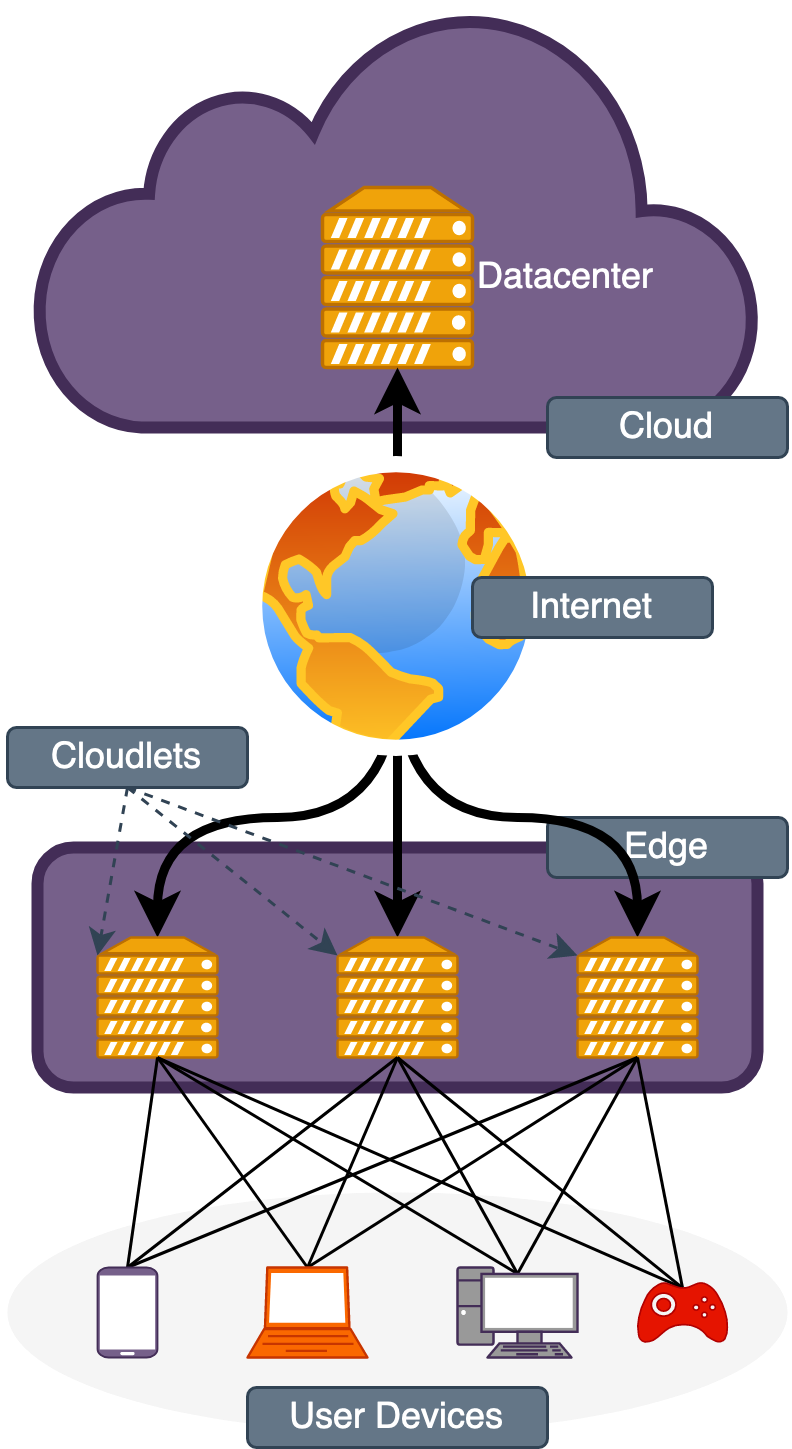
\includegraphics[height=30em]{figures/edgecomputing}
    \caption{%
        Conceptual design of Edge Computing.
        Compute nodes are placed a at the edge of the network, a few hops away from end users.
        In other words, compute is located between users and the internet and the Cloud.
    }\label{fig:edgecomputing}
\end{figure}

Edge Computing aims to improve upon the shortcomings of Cloud Computing by moving the processing closer to the end user, at the \emph{edge} of the network.
In this context, the ``edge of the network'' refers to locations which are both geographically and topologically close to the user, such as micro-datacenters located within the same urban area as the user (see \cref{fig:edgecomputing}).
\gls{MEC}, a variant of the paradigm, even proposes the integration of compute power within 5G~\cite{5Gstandard} cellular networks, co-locating computed nodes with cellular service provider base stations.

By placing computing resources in proximity to where data is generated and/or consumed, and thus reducing the topological and physical distances that data must travel, Edge Computing can greatly decrease latency, improve the responsiveness of applications, and allow for greatly improved efficiency in the use of network resources.
This enables powerful and sophisticated applications to be run on the Edge, such as \glspl{CPS} as well as \gls{XR} applications.
These applications have the potential to have a profound impact in our day-to-day lives, but have stringent latency requirements which make their deployment on traditional paradigms such as Cloud Computing inviable.

\glspl{CPS} refers to systems where physical processes, such as manufacturing or transportation, are controlled  and monitored by computers, usually over communication networks.
Edge Computing allows these systems to operate in real-time, enabling near instantaneous response times, more efficient operation, and more precise control.
These characteristics are critical for applications such as \glspl{ITS}, autonomous driving, or remote surgery.

\gls{XR}, on the other hand, is a broad term that encompasses various forms of immersive application systems.
\gls{XR} applications, such as \gls{AR}, \gls{VR}, or \gls{MR}, involve the real-time interaction between user and virtual elements in a partially to fully immersive environment.
For instance, \gls{MAR} is an application of \gls{AR} that involves overlaying digital information onto the physical world using a mobile device.
This definition has in later years been extended to encompass \gls{AR} deployed on wearable devices (such as Google Glass~\cite{googleglass}) as well.
\gls{MAR} allows users to, for example, view real-time information and details about products while in-store, receive instructions and guidance to perform a complex task, or contextual information while visiting a new city.
By using Edge Computing and 5G, \gls{MAR} --- and other \gls{XR} systems --- can operate with much greater responsiveness and reliability, enabling highly immersive and interactive experiences.

Overall, the combination of Edge Computing and 5G holds great promise for the massive deployment of latency-sensitive applications such as the ones discussed above.
Nonetheless, significant challenges remain in the understanding and scaling of these systems, particularly in regard to their complexity and requirements in the context of low-latency, high-reliability computing.
Before widespread deployment of these systems, it is crucial to thoroughly understand their real-world performance.

\glspl{CPS} often correspond to safety-critical components of industrial systems, and subpar \gls{QoS} can therefore lead to significant danger to equipment and operators.
On the other hand, the immersive nature of \gls{XR} applications implies that poor \gls{QoS} can easily translate into significant user discomfort.
To ensure reliability, safety, and user satisfaction in these systems, careful and accurate characterization and optimization of these systems must be realized.

However, evaluating the performance of such applications on Edge environments represents a significant challenge.
Latency-sensitive applications such as \glspl{CPS} and \gls{XR}, involve multiple processing steps that can influence the latency of the system.
There are many trade-offs involved in optimizing the latency of these applications beyond the question of where the compute process is located. 
These include the choice of wireless system for transmitting application data (e.g.\ 4G \gls{LTE} versus 5G), the protocols used to communicate over the network, and the hardware and operating system used in the backend.
In the case of \gls{XR}, the sensory inputs need to be pre-processed and compressed on-device, before being transmitted to the compute backend for processing.
The backend algorithms need to be carefully designed and implemented to ensure efficient processing and minimal latency. 
Similarly, in \glspl{CPS}, the communication network must be designed to minimize latency and ensure reliable data transmission between the components of the control system.
Other critical aspects with the potential to impact the latency of latency-sensitive applications on the Edge include congestion on the communication loop and fluctuations of the wireless channel.
These issues can lead to delays in data transmission between devices on the network, leading to higher end-to-end latency.

The evaluation of performance in Edge computing systems has been addressed in existing literature through various approaches such as analytical, simulation, and experimental methods.
However, the unique nature of Edge computing environments demands a wide range of interdisciplinary expertise spanning (but not limited to) computer science, communication networks, information theory, queuing analysis, etc.
Such expertise may not always be feasible to obtain within a single research group.
This has led to prior research to often be constrained in its scope, focusing on comprehensive characterization of either compute or network aspects, resulting in potential trade-offs that may neglect one half of the larger picture.
We argue that this limitation has led to an incomplete understanding of the overall performance of Edge systems and applications in the existing literature.
There is a need for holistic approaches that consider both network and compute characteristics of Edge workloads for accurate performance evaluation and optimization.

At the time of the writing of this dissertation, no widely adopted methodology exists for the study of these trade-offs.
We aim to contribute to the field by introducing and subsequently investigating the applications of such a methodology for the study of latency-sensitive applications deployed on Edge infrastructure and network technologies such as 5G.
The proposed methodology aims to enhance the accuracy and realism of results related to Edge infrastructure and 5G networks, particularly in regard to network performance.
Our results will contribute to the development of new techniques and approaches for improving the performance and reliability of \gls{MEC}.

One of the main challenges to the study of latency-sensitive applications such as \gls{CPS} and \gls{MAR} on Edge Computing is that these applications interact with the real world, and thus must be studied in real-time.
This implies that any study of these applications must be done in an environment that accurately reflects the real-world conditions in which they are deployed.
Unfortunately, replicating these conditions in a controlled experimental environment is difficult and often leads to inconsistencies in results, and traditional methods that rely on simulations may not be sufficient to accurately capture and evaluate the performance of these applications in real-world scenarios.

The scalability of studying these systems is also a challenge.
It may not be feasible for researchers to test the applications on a large scale due to limitations in access to specialized equipment, personnel and test subjects, as well as facilities.
\glspl{CPS} often rely on physical sensors and actuators, making it difficult to replicate real-world conditions in a controlled environment at scale, and conducting experiments involving human subjects for \gls{MAR} is time-consuming and expensive.

The highly complex effects on the wireless network is another major challenge to studying latency-sensitive applications on Edge Computing.
The presence of multiple devices accessing the network simultaneously can result in interference, network congestion, and other factors that can affect the performance of the system.
These effects are difficult to simulate and/or emulate, particularly in multi-tenant deployments, where each tenant may have different requirements and resource usage patterns.

Finally, the combination of the characteristics enumerated above makes the study of these applications hard to automate, making it challenging to conduct large-scale experiments or to collect data over an extended period of time.
\gls{CPS} and \gls{MAR} applications are highly dynamic and adaptive, and their behavior cannot be easily predicted.
Moreover, there is often a significant amount of variability in the behavior of different components of the application, such as sensors, actuators, and network connections, which makes it difficult to automate the testing process.

Our methodology is designed to tackle these challenges by employing an emulation approach to the benchmarking of latency-sensitive \gls{CPS} and \gls{MAR} applications. 
We emulate target workloads on actual Edge infrastructure by replacing the client side of the system with \gls{COTS} general-purpose computing devices\footnote{%
    In our initial implementation, these correspond to low-cost and easily replaceable, scalable Raspberry Pi 4 Model B \acsp{SBC}.
} running a realistic software imitation of the desired behaviors.
At the same time, our methodology retains the real network as well as the real compute hardware and software at the backend.
This design results in real-time benchmarking of applications, while still providing realism, scalability, and reduced complexity, as well as allowing for easier automation of these studies.

Emulating the workload component reduces complexity by moving it into the software domain, allowing for easier horizontal scaling through the use of \gls{COTS} general-purpose hardware such as \glspl{SBC}.
This also reduces the barrier of entry to this research, as \glspl{SBC} are for the most part cheap and easily accessible.
Additionally, it preserves the realism of effects stemming from the hardware and network.
In particular, the methodology allows us to capture effects due to network factors such as contention, congestion control, and medium access, which are often of stochastic or chaotic natures and complex to capture in simulations.

The methodology also provides automation as well as improved repeatability and replicability.
The softwarized nature of the client-side emulation allows for straightforward automation through general-purpose programming and scripting languages.
Repeating a study becomes a matter of re-running the workload on the same testbed, and studies can be replicated simply by obtaining the same or equivalent software workload and deploying it on a comparable testbed.
These are complex tasks to accomplish in real-world approaches, particularly when dealing with humans.

We validate our proposed methodology by presenting case studies of its application in two different contexts: \gls{WCA} and \glspl{NCS}.
The case studies demonstrate the efficacy of the methodology in evaluating system performance and overall \gls{QoS} and \gls{QoE}.
Our methodology provides a comprehensive and realistic assessment of the performance of latency-sensitive applications deployed on Edge infrastructure.
The approach provides valuable insights for researchers, system designers, and application developers, and will contribute to the development of new techniques and approaches for improving the performance and reliability of Edge Computing and 5G systems.

In addition to the methodology, this dissertation introduces a number of further contributions to the field. 
We introduce a software framework that facilitates the orchestration of Edge Computing testbeds needed for the implementation of our methodology.
This framework makes it easier for researchers and practitioners to deploy and test Edge-bound low-latency applications.
We also present a deep exploration of this methodology for \gls{WCA} and introduce the first ever model for the end-to-end emulation of human timing behavior in \gls{WCA}.
This model is built from a thorough characterization of these behaviors, the data for which we obtain from a comprehensive human-subject study.

Finally, we explore the implications of our methodology and human user model on the optimization potential of \gls{WCA} deployments.
In particular, we study the sampling and energy consumption behaviors of these systems with and without considering realistic human behavior.
We conclude that significant improvements can be achieved through the use of our human user model.
Overall, our results showcase the utility of our methodology, and the importance of considering human behavior in the design and optimization of \gls{WCA} systems to achieve maximum benefits.

\subsection{Structure of this dissertation}

This dissertation is structured into two parts.
\cref{part:summary} presents a summary of the research, introducing the topic, discussing related work, and highlighting key contributions.
Next, in \cref{part:publications} we present the publications that form the core of this thesis.

\cref{part:summary} is itself structured into four main chapters.
\cref{chap:introduction} serves as an introduction to the topic and outlines the key contributions of this work.
It sets the stage for the subsequent chapters by providing a high-level overview of the research problem and its significance, as well as provides background information on the core topics of the thesis.
In \cref{chap:relwork}, we present the scope of the thesis, as well as relevant related work.
The chapter provides a comprehensive review of the existing literature, highlighting the current state-of-the-art and identifying any gaps in knowledge.
We discuss context for our research, and establish the foundation for the contributions presented in the dissertation.
\cref{chap:contributions} is the core of \cref{part:summary} and provides a detailed summary of the contributions made in this dissertation.
We discuss methods, tools, and findings that were developed and obtained throughout the course of our research.
We aim to demonstrate the significance of our work and how it contributes to the field.
Finally, \cref{chap:conclusions} concludes the dissertation and outlines avenues for future research.
We summarize the key findings and contributions of the thesis, and briefly discuss the implications of our findings and contributions for the field.
This chapter also identifies open questions and areas for further research, providing opportunities to build on the work presented in this thesis.